%% ============================================================================
%%
%%  Master's thesis
%%
%%  Author: FORNAVN EFTERNAVN
%%
%%  Chapter 2: Another topic....
%% ============================================================================

\chapter{BBN code}
\label{chap:BBNcode}

\section{A brief history of BBN codes}
\label{sec:BBN_history}

The concept of Big Bang nucleosynthesis is almost as old as the Big Bang theory itself, with the with it first being proposed in the paper by \textcite{Gamov48}. This early model used neutron capture and subsequent beta decay as the mechanism for BBN, though its greatest problem was the inability to explain the unusually high abundance of oxygen and carbon in the present universe. And so, it was in large part supplanted by the new theory of stellar nucleosynthesis, as the main explanation for the origin of elements. 

During the next decades it became clear that stars could not be the only explanation for the present element abundances, and with the discovery of the CMB in 1965, new attention was brought to the early universe. 
Only a year later Peebles showed how simple BBN physics could be used to explain the high helium abundance, unaccounted for by stellar nucleosynthesis \cite{Peebles66}.

In the following years Wagoner created and refined the first proper BBN code, described in a series of defining papers\cite{Wagoner67}\cite{Wagoner69}\cite{Wagoner72}. With the legacy of this code still heavily influencing the way BBN calculations are performed today.

By the late 80s the Wagoner code was severely outdated. With multiple inefficiencies due to among other things, the fact that it was originally designed to run on punch cards. This inspired Lawrence Kawano to create the now ubiquitous NUC123, colloquially know as the Kawano code\cite{Kawano}. Which set the gold Standard for all future BBN codes. 

\subsection{Modern codes}
\label{sec:newcodes}
In current day and age, there exists multiple publicly available BBN codes, and a countless number of private codes. The most well know of these are PArthENoPE, AlterBBN, and PRIMAT.

PArthENoPE\cite{PArthENoPE} is a spiritual successor to NUC123, and like the works of Wagoner and Kawano PArthENoPE uses FORTRAN. It retains the same structure, and can generally be seen as a continually updated version of these earlier works, with features such as updated reaction rates and a user-friendly GUI.

PRIMAT\cite{PRIMAT} is a Mathematica code and unlike PArthENoPE and AlterBBN, it isn't directly based on the older BBN codes. The main focus of PRIMAT is improving the precision of BBN codes specifically the He4 abundance, which is mainly determined by the $p\leftrightharpoons n$ rates. 

AlterBBN is written in c and based on Kawano's NUC123. It maintains the same basic structure and integration method, though it uses natural units for everything but the reaction network. However, they define energy in GeV rather than MeV. What separates AlterBBN for other codes is that as the name implies, it allows the use of alternate cosmological models and parameters. Therefore, this code is especially well suited for testing the effects these alterations have on final abundances.


\section{Integrating the system of equations}
\label{sec:Solving}

The objective of any BBN code is to solve the system of differential equations described in chapter \ref{chap:theory}, which presents some numerical difficulties. 

Most nuclear reactions have a linear or quadratic dependence on density, as well as an often exponential dependence on temperature. At high temperatures this is balanced by the corresponding reverse rate being equally high. The forward and reverse rates will only cancel at the precise abundance required by nuclear statistical equilibrium (NSE). Any slight deviation from NSE $\delta Y$, will cause one rate to be slightly larger, which due to its magnitude will cause a huge increase in the derivative $Y'$.

Most numerical methods for solving differential equations are explicit, and in their simplest form calculate the next step by adding  $\Delta Y = \Delta t \cdot Y' $. 
If $\Delta Y>2\delta Y$, the system will become unstable as each step will increase the absolute value of both. To avoid this instability an explicit method will have to use a minuscule step size $\Delta t$, which in practice makes the problem unsolvable. 

This and similar problems are called stiff, since they are very inflexible when faced with slight deviations from the "true" solution. 


\subsubsection{Integration methods}

Wagoner and the later codes based on this work handle the stiffness by first linearizing the system, which allows integration in an implicit form:
\begin{align}
    \tilde{Y}_{n+1}=(1+C \Delta t)\tilde{Y}_{n}\approx(1-C \Delta t)^{-1}\tilde{Y}_{n}.
\end{align}
This is then followed by a traditional second order Runge-Kutta integration, with AlterBBN having options for more advanced Runge-Kutta methods. 

PRIMAT on the other hand uses a first order BDF scheme for $T>\num{1.25e9}$ K, switching to second order at lower temperatures for faster computation.

I have chosen to use an implicit Runge-Kutta method of the Radau IIA family of order 5, as implemented in SciPy\cite{SciPy}. This method is perfectly suited to handle stiff problems such as the reaction network, and based on testing it is the most stable method among those available in SciPy.

%Based on my testing this ensures maximum stability, while also being able to utilize the analytical Jacobian derived in equations\eqref{eq:jacterms1}\eqref{eq:jacterms2}.
\subsection{Simplifications of the problem}
Following the example of Wagoner, most BBN codes solve the background variables and abundances concurrently. This is necessary as they account for the change in baryon energy density and electron chemical potential caused by nucleosynthesis. Accounting for the baryon energy only results in a relative abundance change lower than $10^{-5}$ for the heavier nuclei, and even less for lighter ones. Accounting for baryons at all is questionable, and tracking the abundance of non-thermal electrons and energy changes caused by nucleosynthesis is completely unnecessary. Accordingly, the background variables can be treated as independent of the abundances.

This is beneficial, as unlike the abundances the equations governing temperature and scale factor are not stiff in the slightest. This allows faster integration, with fewer evaluations of computationally demanding terms such as the sum in electron energy density \eqref{eq:rhoelectron}. Barring $e^-$ $e^+$ annihilation, $T$ and $a$ follow the simple power laws $T^{-2}\propto t$ and $a^2\propto t$, as seen on figure \ref{fig:Temperature}. This allows the use of simple linear interpolation in log space, which will have negligible impact on runtime compared to the evaluation of reaction rates.

Compared to the background parameters, evaluating reaction rates is quite simple, with the most time-consuming part being the sheer number of rates, which can be mitigated somewhat with parallelization. Here the main problem is the aforementioned stiffness, but this is also aided by precomputing the background variables, as this demonstrably improves stability. 




\section{Creating the reaction network}
\label{sec:pna}
To create the reaction network I use pynucastro\cite{pynucastro2}, which is an open source python interface designed for nuclear astrophysics. The reaction rates themselves are provided by the REACLIB database\cite{REACLIB}. These rates are based on fits of experimental results using the following parametrization 
\begin{align}
    \lambda = \exp\left(a_0+\sum_{i=1}^{5}a_i T_9^{\frac{2i-5}{3}}+a_6 \log{T_9}\right).
    \label{eq:reacliblambda}
\end{align}
T9 is the temperature in \num{1e9} K, and the molar density must be provided in cgs units of $\text{mol}/\text{cm}^3$. Converting from natural units to cgs is a simple matter of multiplying by $\frac{MeV}{\hbar c}^3\frac{1}{N_0}=\SI{2.161e8}{\cm^{-3}}$, with $N_0$ being the Avogadro number. For some reactions such as those with powerful resonances, a rate can be comprised of multiple terms of the form given in \eqref{eq:reacliblambda}, to allow for more accurate fit of the data. 

To create the network, pynucastro must first be provided with the list of included nuclei. It has a built-in method for collecting all reactions between these nuclei which creates a library object containing the rates and their relations. This can then be used to generate a python file which takes density, temperature and abundances as inputs and returns the rhs and Jacobian. This file supports just in time compilation using the JIT module from Numba, which takes between a few seconds to a few minutes depending on the size of the network. To avoid having to compile the networks every time I modify the code, I added a method that compiles the network ahead of time using the Numba CC module. 

At high temperatures heavy nuclei have extremely low abundances while greatly increase the stiffness of the system. To increase both stability and performance, it is prudent to extend the network gradually, which can be accomplished by using 3 different reaction networks. 

At very high temperatures, deuterium is readily destroyed by high energy photons inhibiting the production of any subsequent nuclei. Here the simplest possible reaction network is employed, comprised of only the proton, neutron, their forward and reverse rate. 

When temperatures are low enough to allow deuterium production then network is extended to include all nuclei with $A\leq 7$, see figure \ref{fig:smallnet}. This accounts for the nuclei involved in ${}^4$He production and their immediate fusion products, which are also the only nuclei with observable final abundances. 

\begin{figure}[ht]
    %\centering
    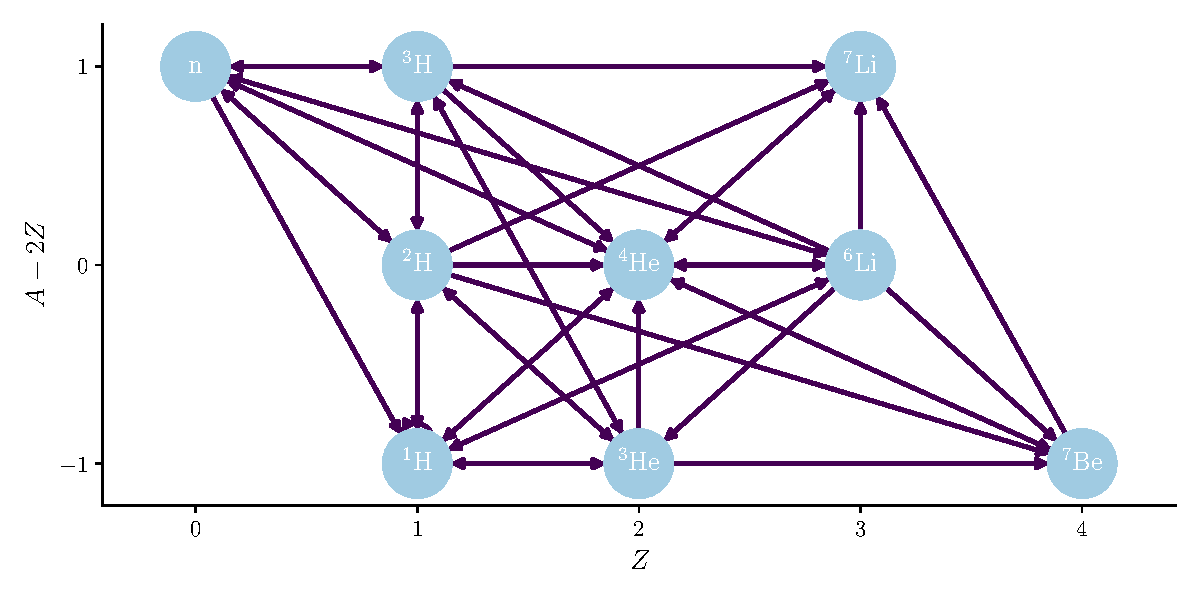
\includegraphics[width=5.1in]{figures/lillenet.pdf}
    \caption{Reduced reaction network for calculating light element abundances at high temperatures, with arrows representing forward reaction rates}
    \label{fig:smallnet}
\end{figure}

When significant amounts of ${}^4$He and heavier nuclei have formed, we switch to the full network which includes every nucleus that could possibly affect BBN, see figure \ref{fig:bignet}. Due to the extreme temperature dependence of reactions such as triple alpha, this network is very stiff at high temperatures. 

\begin{figure}[ht]
    %\centering
    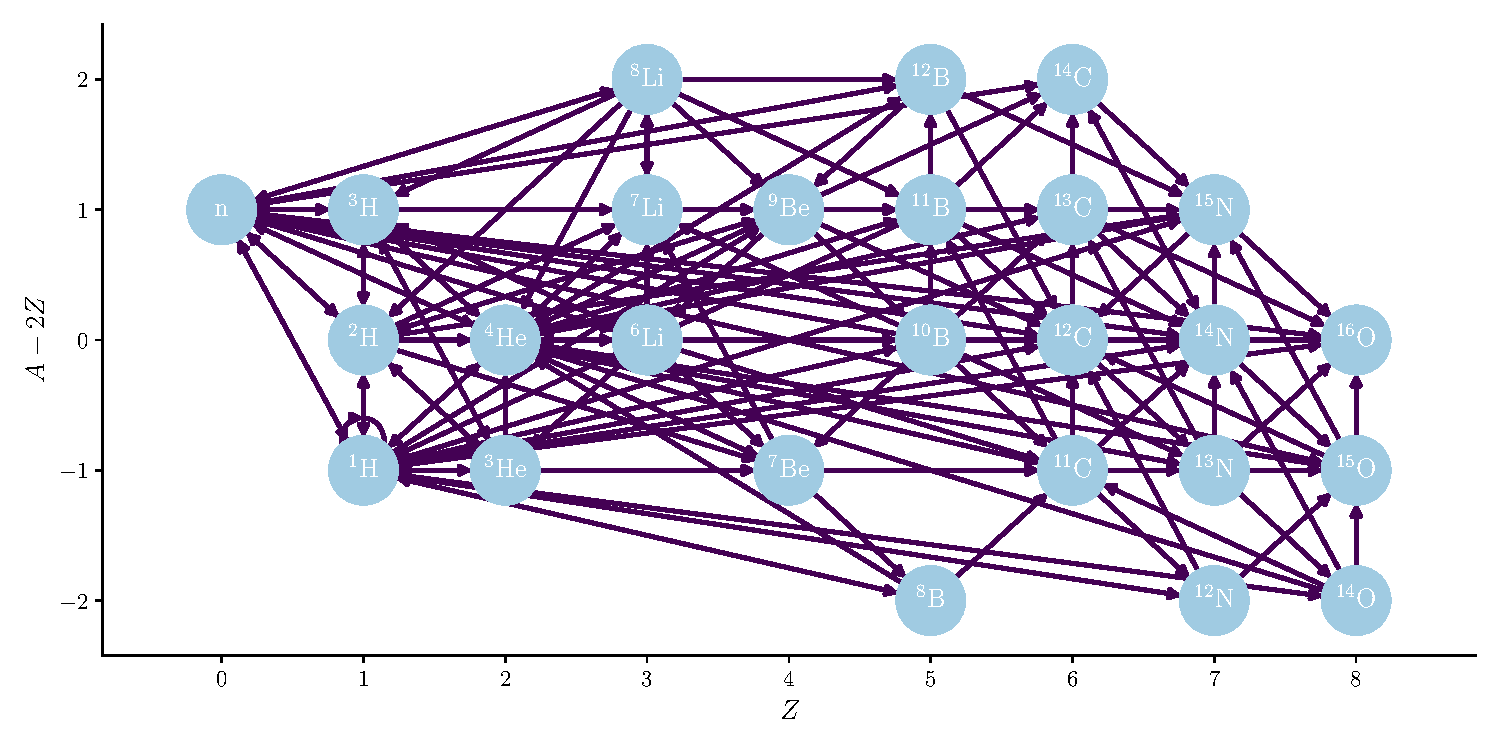
\includegraphics[width=5.1in]{figures/stornet.pdf}
    \caption{Full reaction network for more precise determination of heavy element abundances at intermediate to low temperatures, with arrows representing forward reaction rates}
    \label{fig:bignet}
\end{figure}

\section{Running the code}
\label{sec:structure}

\begin{itemize}
    \item We use pynucastro to generate the reaction networks. This is by far the most time-consuming step, but unless we need to modify a reaction rate, we only need to do it once.
    \item The time evolution of background parameters is calculated and stored. To speed up subsequent calls to the background parameters, JIT is use for the interpolation function.
    \item Initial conditions are set based on the background parameters, with the proton and neutron abundance being determined from NSE.
    \item The first reaction network is integrated, from a specified initial time until the switch to the second network. 
    \item Before beginning integration the second network, the initial abundance of the added nuclei is determined by requiring that the resulting right-hand-side (RHS) is 0. This minimizes the transients created as the new nuclei rapidly readjust due to the stiffness of the system.
    \item The second reaction network is integrated using these initial conditions, after which the same procedure is used for the third network.
    \item Barring the addition of additional reaction networks, we get the final abundances, as well as their evolution over time.
\end{itemize}

